\chapter{Tensor Structured Coupled Cluster
\label{ch:tcc}} 
The discussion presented in this section is based on our published work, see 
Ref.~\cite{schutski2017tensor}, and also on several new results intended for 
another publication.

In this chapter we will discuss in more detail the steep scaling of coupled 
cluster. To remedy this scaling we use the concept of tensor decompositions, and 
we will review several relevant decompositions 
in Sections~\ref{sec:canonical_decomposition} and 
\ref{sec:tensor_hypercontraction}. A general way to optimize tensor 
decompositions in mentioned in Section~\ref{sec:als}. 
Section~\ref{sec:tcc_derivation} explains how we can combine tensor 
decompositions with coupled cluster. The last section is an 
appendix introducing the diagrammatic notation we use to schematically display 
our main results.

\section{Tensor Contractions and the Cost of Coupled Cluster}
Our goal here is to improve the very steep cost of the coupled 
cluster method. The numerical cost of CC methods lies in solving amplitude 
equations. We will show how to reduce this effort by two orders of 
magnitude by introducing alternative representations of the Hamiltonian 
and amplitude tensors. But first, let us look back at some of the terms in the 
RCCD amplitude equation:
%
\begin{equation}
\begin{split}
T^{ab}_{ij} & = D^{ab}_{ij} \cdot (- V^{ab}_{ij} \\
& + \sum_{k \neq i} F^{k}_{i} T^{ab}_{kj}
+  \sum_{k \neq j} F^{k}_{j}  T^{ab}_{ik}
- \sum_{c \neq a} F^{a}_{c}  T^{cb}_{ij}
- \sum_{c \neq b} F^{b}_{c}  T^{ac}_{ij} \\
& - T^{cd}_{ij}  V^{ab}_{cd}
+ T^{ac}_{ik}  V^{bk}_{cj} 
+ T^{ac}_{ki}  V^{bk}_{jc} 
+ T^{ac}_{kj}  V^{bk}_{ci} 
+ T^{bc}_{jk}  V^{ak}_{ci}\\
&+ \mathrm{other~terms}
\end{split}
\label{eq:ccd_amplitude_equation_head}
\end{equation}
%
Again, here $F$ is the Fock matrix, $V$ is the electron interaction tensor in 
the molecular orbital basis (Dirac ordered) and $D$ is an orbital energy 
denominator. Most of the terms on the right hand side of 
Eqn.~\ref{eq:ccd_amplitude_equation_head} are numerically expensive to 
evaluate. For example, the second term containing interaction 
$V$ is
%
\begin{equation}
 \tau^{ab}_{ij} = T^{ac}_{ik}  V^{bk}_{cj}
 \label{eq:ccd_intermediate_example}
\end{equation}
%
This expression requires $O(N^6)$ multiplications and additions, as for every 
one of the $N^4$ elements in the intermediate $\tau$ one has to calculate $N^2$ 
products and sums. To facilitate the discussion and the estimates of cost let 
us introduce a graphical notation for tensors:
%
\begin{equation}
\vcenter{\hbox{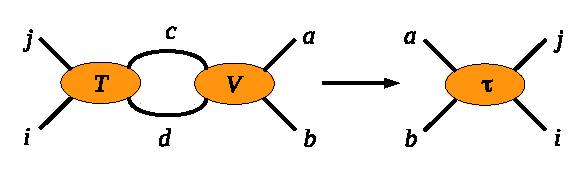
\includegraphics[width=0.6\textwidth]
{figures/tcc_theory/cc_contraction_1} } }
.
\label{fig:cc_contraction_1}
\end{equation}
%
In this notation we represent tensors by shapes, and their 
indices by lines. Open lines denote free indices, and connected lines mean a
contraction over respective indices. If each index had a size proportional to 
$N$, one can then estimate the cost of the contraction as $N^{K}$, where the 
exponent $K$ is the sum of the number of open lines in the result and 
the number of connected lines. Thus, the cost scales as $N^6$ in 
Eqn.~\ref{fig:cc_contraction_1}. For more examples of the graphical notation 
please see Appendix~\ref{sec:graphical_notation}. We will omit index 
letters on most further diagrams.

The very same contraction can be evaluated with lesser effort if the electron 
interaction tensor is approximated by a well known\cite{beebe1977, 
vahtras1993integral, boman2008method, sierka2003fast} resolution of identity 
(RI) decomposition:
%
\begin{equation} V^{pq}_{rs} \approx \sum_{\alpha \alpha^{\prime}} 
U_{pr}^{\alpha}
D_{\alpha,\alpha^{\prime}} \tilde{U}_{qs}^{\alpha^{\prime}},
\label{eq:ri_decomposition}
\end{equation}
Here $U$ and $\tilde{U}$ are three index-integrals and $D$ is a generalized 
overlap.\cite{ahmadi1995coulomb}. The resolution of identity can be 
seen as a singular value or an eigenvalue decomposition of the 
interaction tensor. The tensor $V^{pq}_{rs}$ can be seen as matrix 
$V(pr, qs)$ with combined indices $pr$ and $qs$. The three index tensors $U$ and 
$\tilde{U}$ are its singular vectors (or eigenvectors), and $D$ is a diagonal 
matrix of singular values (or eigenvalues). The RI decomposition, however, does 
not enforce in general that $U$ and $\tilde{U}$ are orthogonal or that $D$ is 
diagonal.

The accuracy of the decomposition in Eqn.~\ref{eq:ri_decomposition}
will depend on the size of the introduced index $\{ \alpha \}$, called the rank 
of RI, or the size of the auxiliary basis. It is well known that the error of 
RI decreases exponentially with the size of $\{ \alpha \}$. Negligible errors 
are attained with $dim(\{ \alpha \}) = r_{RI} = O(N)$.\cite{beebe1977, 
sierka2003fast} Diagrammatically, Eqn.~\ref{eq:ri_decomposition} is
%
\begin{equation}
\vcenter{\hbox{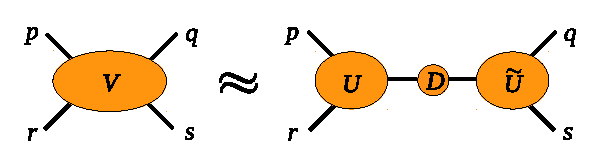
\includegraphics[width=0.6\textwidth]
{figures/tcc_theory/ri_decomposition}}}.
\label{fig:ri_decomposition}
\end{equation}
%
By using the RI decomposition the intermediate in 
Eqn.~\ref{fig:cc_contraction_1} can be formed at $O(N^5)$ cost, 
as shown on the diagram below:
%
\begin{equation}
\vcenter{\hbox{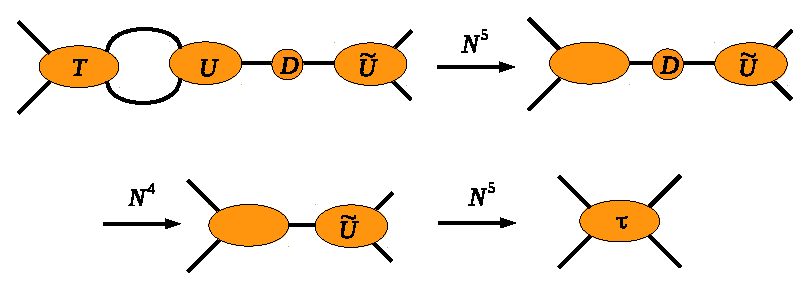
\includegraphics[width=0.6\textwidth]
{figures/tcc_theory/cc_contraction_2}}}.
\label{fig:cc_contraction_2}
\end{equation}
%
The RI decomposition has been used for a long time to reduce the
scaling of quantum chemistry algorithms, for example, in the RI-MP2
method.\cite{ayala1999linear, werner2003fast, izmaylov2008resolution} A 
significant caveat is, however, that indices of $V^{pq}_{rs}$ can be 
separated by RI only in a specific order. If $V$ is seen as a matrix 
$V(pr, qs)$, which we refer to as Mulliken order, then pairs of 
indices $pr$ and $qs$ can be separated with good accuracy at low rank 
$r_{RI}$. In contrast, if we cast $V$ into a matrix 
$V(pq,rs)$, which we refer to as Dirac order, and try to separate
$pq$ from $rs$, then the rank of RI has to be $r_{RI} = O(N^2)$ to provide 
equivalent accuracy. The approximation in the last 
case would be not useful, because RI factors would contain almost the same 
number of elements as the original tensor. Those 
properties of RI are apparent from the form of the electron interaction 
operator:
%
\begin{equation}
%\begin{split}
 V^{pq}_{rs} = \int \frac{\phi^{\star}_{p}(\vec{r}_{1}) 
\phi^{\star}_{q}(\vec{r}_{2}) \phi_{r}(\vec{r}_{1}) \phi_{s}(\vec{r}_{2})}{| 
\vec{r}_{1} - \vec{r}_{2} |} 
d\vec{r}_{1} d\vec{r}_{2} \\ 
%& \approx \int \phi^{\ast}_{p}(r_{1}) \phi_{r}(r_{1}) \chi_{\alpha}(r_{1}) 
%dr_{1} 
%\int \phi^{\ast}_{q}(r_{2}) \chi_{s}(r_{2}) \psi_{\alpha^{\prime}}(r_{2}) 
%dr_{2} \\ & \cdot \int \frac{\chi_{\alpha}(r_{1}) 
%\chi_{\alpha^{\prime}}(r_{2})}{| r_{1} - 
%r_{2} |} dr_{1} dr_{2}
%\end{split}
\label{eq:ri_decomposition_integral}
\end{equation}
%
As Eqn.~\ref{eq:ri_decomposition_integral} implies, a separation of variables 
between a pair of basis functions $p, r$ and $q, s$ is possible when the 
distance $|\vec{r}_{1} - \vec{r}_{2}|$ is large. In contrast, this is not true 
for pairs $p, q$ and $r, s$ in $V^{pq}_{rs}$.

This limitation of the RI decomposition does not allow cost reduction during 
the calculation of several terms in the residual equation of RCCD. For example, 
the evaluation of the 6th term Eqn.~\ref{eq:ccd_amplitude_equation}:
%
\begin{equation}
 \tau^{ab}_{ij} = - T^{cd}_{ij}  V^{ab}_{cd}
 \label{eq:ccd_intermediate_example2}
\end{equation}
%
does not benefit from RI decomposition of $V$.
%
\begin{equation}
\vcenter{\hbox{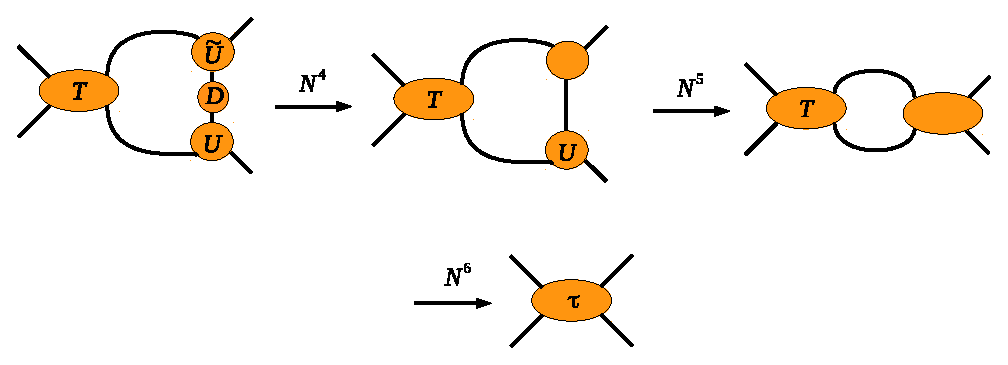
\includegraphics[width=0.8\textwidth]
{figures/tcc_theory/cc_contraction_3}}}
.
\end{equation}
%
Further approximations, however, can lead to lower cost of this expression.

\section{Tensor decompositions}
As was noted before, the simple RI approximation may not always reduce the 
computational cost. To build a more flexible approximation of the interaction 
tensor we need to consider additional tensor decompositions. In this section we 
will only briefly list the decompositions we used, and refer the reader to 
the original publications for technical details. The important information here 
is the structure of the described factorizations, which we demonstrate using 
tensor diagrams. Another important aspect is the alternating least squares 
method (ALS), as it can be used to calculate \emph{any} of the described 
decompositions and is a cornerstone of our factorized CC approaches.

\subsection{Canonical Polyadic Decomposition
\label{sec:canonical_decomposition}}
An $n$-dimensional tensor can always be produced as a result of the direct 
product of $n$ vectors. In the simplest case of the three dimensional tensor 
with one vector per each dimension we would have:
%
\begin{equation}
\tau = a \times b \times c 
\end{equation}
%
These tensors are called elementary rank-1 tensors or polyads. The Hartree-Fock 
method can be regarded as minimization of the energy functional over 
wavefunctions being a single polyad (over antisymmetric vector spaces and with 
an additional constraint of vectors to be orthogonal and normalized). General 
tensors, however, can be expressed as sums 
of polyads~\cite{hackbusch2014numerical} 
(again, compare this to correlated wavefunctions in many-body theory, which may 
be expressed as sums of Slater determinants):
%
\begin{equation}
 T = \sum_{\alpha} \tau^{\alpha}
\end{equation}
%
The polyadic decomposition~\cite{de2006link} of a tensor is thus a decomposition 
of the form:
%
\begin{equation}
T_{pqr\ldots} = \sum_\alpha a_p^\alpha \, b_q^\alpha \,
c_r^\alpha \ldots
\label{eq:cpd_definition}
\end{equation}
%
The dimension of the auxiliary index $\alpha$ is called the 
rank of the decomposition. As the rank is increased, this decomposition can 
approximate an arbitrary tensor with any given precision. The factorization with 
the lowest possible rank is called canonical polyadic decomposition (CPD), but 
we would omit this detail and call CPD any decomposition of the form shown in 
Eqn.~\ref{eq:cpd_definition}. The CPD of a three index tensor is shown below 
diagrammatically.
\begin{equation}
\vcenter{\hbox{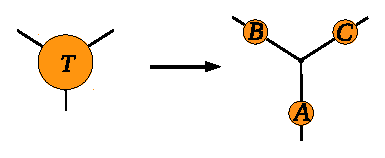
\includegraphics[width=0.4\textwidth]
{figures/tcc_theory/cp_decomposition}}}
.
\label{fig:cp_decomposition}
\end{equation}
%
This factorization can be seen as one of the generalizations of classic 
decompositions of matrices, such as QR, LU or Singular Value Decomposition, to 
higher order tensors.\cite{kolda2009tensor} The important 
difference, is, however, that no closed form algorithm to extract the CPD for 
generic tensors is known, and one has to rely on iterative optimization 
techniques.\cite{sorber2013optimization} 

Substantial effort has been made by the mathematical community to develop 
optimization techniques for CPD. We refer the reader to the corresponding 
reviews~\cite{kolda2009tensor, sidiropoulos2016tensor} for further details. 
Typical algorithms are the alternating least squares 
(ALS),\cite{comon2009tensor} gradient descent by 
means of the method of Broyden, Fletcher, Goldfarb, and Shanno 
(BFGS), and nonlinear least squares (NLS) methods.\cite{sorber2013optimization}

\subsubsection{Analytical Canonical Decomposition}
For a limited number of special tensors the CPD can be built analytically. 
One such case are tensors which can be expressed in the form:
%
\begin{equation}
T_{abc\ldots} = 
f(x_{a} + y_{b} + z_{c} + \ldots)
\end{equation}
%
Here $f$ is an arbitrary differentiable function, and $x_{a}$ are values of the 
argument on a finite interval. CP decomposition for these tensors can be 
built using an exponential parameterization.\cite{braess2005approximation} We 
note that the denominator tensors in coupled cluster theories (see Section 
\ref{sec:preliminaries_rccd}) have a suitable structure: 
%
\begin{equation}
D^{ab\ldots}_{ij\ldots} = 
\frac{1}{F_{a}^{a} + F_{b}^{b} + \ldots - F_{i}^{i} - 
F_{j}^{j} - \ldots}
\end{equation}
CPD of energy denominator tensors was known as Laplace 
transformation in quantum chemistry for a long 
time.\cite{almlof1991elimination} The exponential parameterization of the 
denominator tensors is:
%
\begin{subequations}
\begin{align} {}^2D_{ij}^{ab} &= 
\sum_{\omega} C_\omega \, \mathrm{e}^{A_\omega \,
F_i^i} \, \mathrm{e}^{A_\omega \, F_j^j} \, \mathrm{e}^{-A_\omega \,
F_a^a} \, \mathrm{e}^{-A_\omega \, F_b^b} \\ &= \sum_{\omega} {}^2D^1_{i,\omega} 
\,
{}^2D^2_{j,\omega} \, {}^2D^3_{a,\omega} \, {}^2D^4_{b,\omega}.
\end{align}
\end{subequations}
%
Quadrature weights $C_{w}$ and coefficients $A_{w}$ in this case can be 
precomputed without knowledge of the individual values of the Fock matrix 
diagonal $F$ (they depend only on the span of the values and a desired 
magnitude of error) and provide very high accuracy of the resulting 
decomposition.\cite{braess2005approximation}
%
\subsubsection{Exact decomposition of sparse tensors}
Another important special case when an exact CPD can be built are very sparse 
tensors. A tensor $T$ having $r$ non zero elements can be represented exactly 
by its trivial CPD of rank $r$, which will take a form
%
\begin{equation}
T_{pqr\ldots} = \sum_{\alpha \in T_{pqr\ldots} \neq 0} \lambda_{p^\alpha 
q^{\alpha} 
r^{\alpha}\ldots} \cdot e^{1}_{p^{\alpha}} \, e^{2}_{q^\alpha} \, 
e^{3}_{r^\alpha} \ldots
\label{eq:trivial_cpd_dec}
\end{equation}
%
where $e^{n}_{p^{\alpha}}$ is a unit vector of the same length as $n$-th 
dimension of $T$ having $1$ in $p^{\alpha}$-th position, and 
$\lambda_{p^{\alpha}q^{\alpha}r^{\alpha}\ldots}$ is a non-zero element of 
$T$. Essentially, CPD in this case is a weighted sum of rank-1 tensors having 
$1$ in a specific entry and 
zeros everywhere else with 
weights corresponding to the values of non-zeros entries in $T$. This 
trivial decomposition may be useful only if the number of non-zero entries of 
$T$, and hence the rank of the CPD, is small. The particular way this trivial 
CPD is built shows an intrinsic connection of the CPD and sparsity.

\subsection{Tensor Hypercontraction
\label{sec:tensor_hypercontraction}}
The resolution of identity, which we considered before, can be combined with 
canonical decomposition. If the three-index tensors in RI 
are further approximated by CPD one comes to a Tensor Hypercontraction (THC) 
introduced by Martinez \emph{et al.}\cite{hohenstein_thc1, hohenstein_thc2, 
hohenstein_thc3} The THC is a decomposition of fourth order tensors of the form:
\begin{equation}
\begin{split} V_{pqrs} & = \sum_{\alpha \beta} W^{1}_{p,\alpha} W^{2}_{q, 
\alpha}
X_{\alpha, \beta} W^{3}_{r, \beta} W^{4}_{s, \beta} 
\end{split}
\label{eq:thc_definition}
\end{equation}
Diagrammatically, THC is
\begin{equation}
\vcenter{\hbox{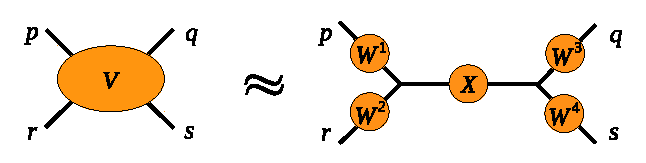
\includegraphics[width=0.5\textwidth]
{figures/tcc_theory/thc_decomposition}}}
.\label{fig:thc_decomposition}
\end{equation}
THC can be seen as a further approximation to RI, which is apparent from the 
following sequence of diagrams:
\begin{equation}
\vcenter{\hbox{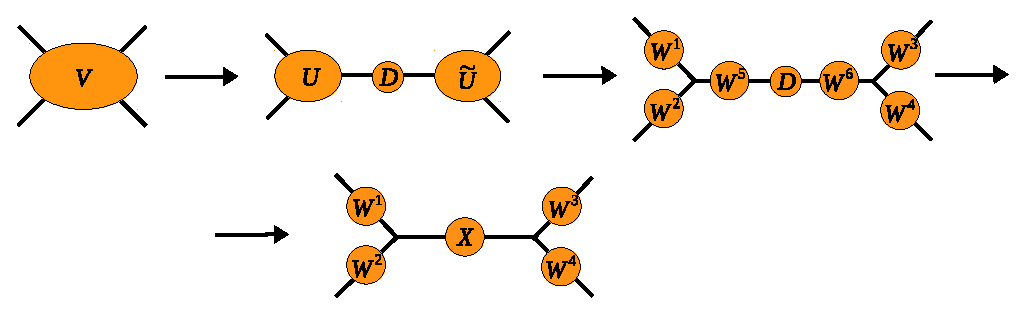
\includegraphics[width=0.8\textwidth]
{figures/tcc_theory/thc_cpd}}}.\label{fig:thc_cpd}
\end{equation}
As those diagrams suggest, THC can be calculated in two steps. First, an RI 
of the original tensor is calculated, and then CP decomposition of the 
three-index tensors is obtained by means of optimization 
algorithms. Finally, the factors without external indices (open lines) 
are contracted together to produce the THC.\cite{hohenstein_thc1}
Let us also note that the order of indices affects the accuracy of THC in the 
same way as in case of RI. We use Mulliken ordering for all THC decomposed 
tensors in this work. 

For the specific case of two electron integrals Martinez \emph{et al.} developed 
fast non-iterative methods where fixed real-space quadratures were used in 
place of factors $W^{1}, W^{2}, W^{3}, W^{4}$.\cite{hohenstein_thc3, 
hohenstein_cc2, parrish2013discrete} This can be compared to obtaining CPD 
analytically, as was mentioned in the previous section.

We also proposed direct optimization methods for calculating THC by alternating 
least squares and gradient descent in our work,\cite{schutski2017tensor} but 
found them inferior to the two step approach originally described by Martinez 
\emph{et al.}.\cite{hohenstein_thc1}

\section{Alternating Least Squares
\label{sec:als}}
Let us now describe a general optimization method, which can be applied to 
calculate several tensor decompositions. We will show its derivation for the 
optimization of THC as was done in our original work,\cite{schutski2017tensor} 
but it can be equally used to compute CPD and, possibly, other decompositions.

We start by defining an approximation to a four index tensor $V$ by its THC 
decomposition $\tilde{V}$:
%
\begin{subequations}
\begin{align} \tilde{V}_{ijkl} &= \sum_{\alpha \beta} W^{1}_{p,\alpha} W^{2}_{q, 
\alpha} X_{\alpha, \beta} W^{3}_{r, \beta} W^{4}_{s, \beta} \\
\end{align}
\end{subequations}
%
The element-wise error can be written as
%
\begin{equation}
\Delta_{V} = V - \tilde{V},
\end{equation}
%
the square of the Frobenius norm of this tensor is a sum of its entries squared:
%
\begin{equation} f = \|\Delta_V\|^2 = \sum_{pqrs} \left(V^\ast_{pqrs} -
\tilde{V}^\ast_{pqrs}\right) \, \left(V_{pqrs} -
\tilde{V}_{pqrs}\right).
\label{eq:cost_function}
\end{equation}
%
Diagrammatically, the latter expression is
%
\begin{equation}
\vcenter{\hbox{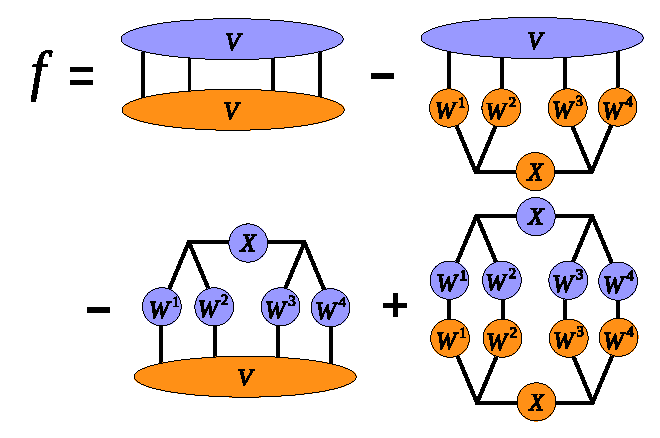
\includegraphics[width=0.5\textwidth]
{figures/tcc_theory/cost_function} } } .
\label{fig:cost_function}
\end{equation}
%
where we denoted conjugated tensors by darker color. Clearly, the best possible 
THC approximation to $V$ will correspond to a minimum of the cost function $f$. 
Since $f$ is a real-valued analytic function, its derivatives with respect to 
possibly complex factors $W \in \{W^1, W^2, W^3, W^4, X\}$ are related by
$\frac{\partial f}{\partial W} = (\frac{\partial f}{\partial W^{\ast}})^{\ast}$.

In order to minimize the cost function, we proceed with the
calculation of its gradient, which can be easily done using
diagram~\ref{fig:cost_function}.  The partial derivative of $f$ with
respect to $W^1$ is
%
\begin{equation}
\vcenter{
\hbox{
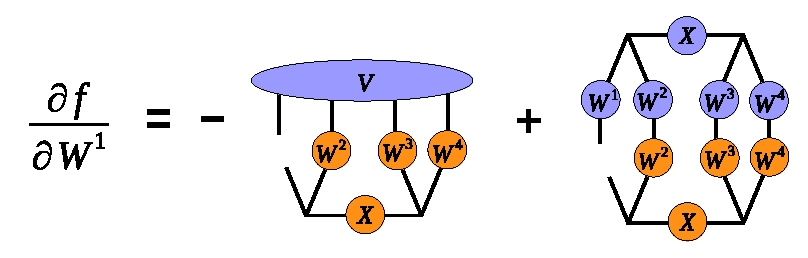
\includegraphics[width=0.7\textwidth]
{figures/tcc_theory/cost_function_dfdw1}}}
\label{fig:cost_function_partial}
\end{equation}
%
Likewise, partial derivatives of $f$ with respect to other factors are 
expressed by similar diagrams with those factors removed. Using the fact that 
$\frac{\partial f}{\partial W}$ is linear in $W^\ast$, we can contract all 
factors around $W^\ast$ into an environment matrix $A$, as shown in 
diagram~\ref{fig:least_squares_w1}, and set this derivative to zero:
%
\begin{equation}
\vcenter{\hbox{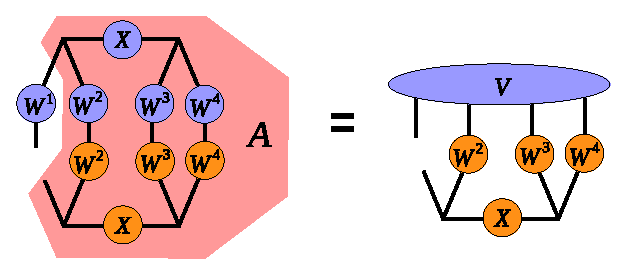
\includegraphics[width=0.5\textwidth]
{figures/tcc_theory/least_squares_w1} } }
\label{fig:least_squares_w1}
\end{equation}
%
We end up with a problem
%
\begin{equation}
A \cdot W^\ast = B.
\label{eq:least_squares_w1}
\end{equation}
%
The solution to Eqn.~\ref{eq:least_squares_w1} can be
obtained by multiplying from the left by the inverse of $A$ (or a 
pseudoinverse, if $A$ is a rank-deficient matrix).  Finally, we arrive to an 
expression for ${W^{1}}^{\ast}$, which diagrammatrically is
%
\begin{equation}
\vcenter{
\hbox{
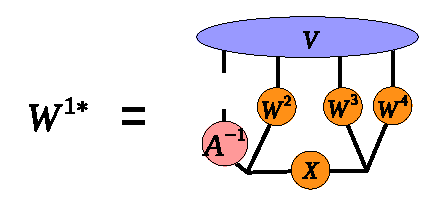
\includegraphics[width=0.4\textwidth]
{figures/tcc_theory/least_squares_w1_sol}}}
 .
\label{fig:least_squares_w1_sol}
\end{equation}
%
Let us estimate the cost of this procedure. We call the size of the 
auxiliary indices $\alpha, \alpha^{\prime}$ the rank of the THC 
decomposition ($r_\mathrm{THC}$). The construction of the environment 
matrix $A$ scales as $O(r_\mathrm{THC}^3)$, as does computing its generalized 
inverse. If each of the dimensions of $V$ equals $N$, then the cost of 
calculating ${W^1}^{\ast}$ scales as $O(N^4 \, r_\mathrm{THC})$. Updates for the
rest of the terms in the THC decomposition can be calculated similarly.

A simple iterative optimization algorithm can be built as follows.
First, the THC factors $W$ are initialized randomly.  For each factor,
an update is calculated as shown on diagram~\ref{fig:least_squares_w1_sol}, 
keeping the other factors fixed.  The process is iterated until convergence of 
the factors. We note that this procedure is, in fact, very similar to 
partial gradient descent and the Gauss-Siedel method.\cite{yoon1988lower} The 
resulting THC-ALS algorithm is listed below.
%
\begin{algorithm}[H]
  \caption{Alternating Least Squares}\label{code:thc_als}
  \begin{algorithmic}[1] 
  \Function{thc-als}{$V, r_\mathrm{THC}, \epsilon$}
  \State $I_{1},I_{2},I_{3},I_{4} \gets$ size($V$)
  \State $W^1, W^2, W^3, W^4, X \gets$ init\_random($I_{1}, I_{2}, I_{3}, 
I_{4}, r_\mathrm{THC}$) 
  \Repeat \ForAll {$W \in \{W^1, W^2, W^3, W^4,
X\}$}
  \State $A_{W} \gets $ get\_environment($W^1, W^2, W^3, W^4, X$)
  \LineComment{$O(r_\mathrm{THC}^3)$}
  \State $B_{W} \gets $ get\_rhs($V,
   W^1, W^2, W^3, W^4, X$) \LineComment{$O(N^4 \, r_\mathrm{THC})$ or
$O(N^2 \, r_\mathrm{RI} \, r_\mathrm{THC})$ with RI}
   \State $W_{new} \gets A^{-1} B$\Comment{$O(r_\mathrm{THC}^3)$}
   \EndFor
   \State $\Delta \gets \max_{W} \frac{\| W_{new} - W \|}{\|
W \|}$
   \State $W \gets W_{new}$ 
   \Until $\Delta > \epsilon$ 
   
   \Return $W^1, W^2, W^3, W^4, X$
    \EndFunction
  \end{algorithmic}
\end{algorithm}
%
The calculation of the right hand side of
Eqn.~\ref{eq:least_squares_w1} dominates in the cost of THC-ALS,
scaling as $O(N^4 \, r_\mathrm{THC})$. A simple modification is
possible to reduce the cost of this step by one order of magnitude. If an
RI approximation to the original tensor $V$ is available from the beginning, as 
in the case of the electron interaction, it can be used in place of $V$, 
leading to a faster algorithm. The diagram corresponding to 
Eqn.~\ref{eq:least_squares_w1} then becomes
%
\begin{equation}
\vcenter{\hbox{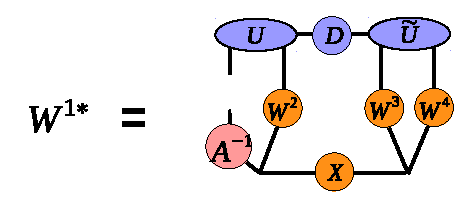
\includegraphics[width=0.4\textwidth]
{figures/tcc_theory/least_squares_w1_sol_ri} } }
\label{fig:least_squares_w1_sol_ri}
\end{equation}
%
The cost of the expression above scales as $O(N^2 \,
r_\mathrm{RI} \, r_\mathrm{THC})$, because the contraction of a
fourth-index tensor $V$ with matrices $W$ is replaced by contractions
of two third-index tensors $U$ and $\tilde{U}$. We only need to
modify the function $get\_rhs()$ in the Algorithm~\ref{code:thc_als} to build a 
lower scaling algorithm,
which we refer to as THC-ALS-RI.

Alternating least squares algorithms are simple and 
often robust,\cite{uschmajew2012local} but may take a large number of
iterations to converge.\cite{comon2009tensor} Particularly, we found that 
calculating THC decomposition with ALS directly is inferior to using a two 
step scheme mentioned earlier.\cite{schutski2017tensor} Nevertheless, the ALS 
procedure can be derived for various decompositions, and is a cornerstone of 
our tensor structured coupled cluster.

\section{Tensor Structured Coupled Cluster
\label{sec:tcc_derivation}}
The ALS algorithm can be merged together with CC equations, leading to
CC expressions with significantly lower computational cost, which are the main 
achievement of our work.\cite{schutski2017tensor} The logic of deriving those 
novel approaches follows the same route as in the case of the ALS method. Here, 
we will use coupled cluster doubles (for which one neglects ${}^1\hat{T}$) as as 
example, and THC decomposition of all four index tensors. This scheme, 
however, is quite general, and we have applied it to other decompositions and 
coupled cluster methods, as discussed in subsequent sections. 

Let us impose the THC structure on the doubles amplitudes. We
approximate the amplitude tensor ${}^{2}T$ with its THC decomposition
${}^{2}\tilde{T}$ having rank $r_{T}$.  The difference between the original and 
approximated amplitudes is
%
\begin{equation} 
\Delta_{T} = {}^{2}T - {}^{2}\tilde{T} = {}^{2}T -
(Y^{2} \odot Y^{1}) \cdot Z \cdot (Y^{4} \odot Y^{3})^{T},
\end{equation}
%
where $Y^{i}$ and $Z$ are factor matrices in the THC
decomposition of ${}^{2}T$. As in the case of the ALS algorithm, we wish to 
minimize the squared norm of the error tensor $\Delta_{T}$, which is the 
minimization of 
the corresponding cost function $f_{T}$,
%
\begin{equation}
f_{T} = |\Delta_{T}|^2 = ({}^{2}T^{\ast} -
{}^{2}\tilde{T}^{\ast})({}^{2}T - {}^{2}\tilde{T}).
\end{equation}
%
Setting partial derivatives of $f_{T}$ with respect to
the decomposition factors to zero, we obtain a new set of equations
%
\begin{equation} 
\frac{\partial f_{T}}{\partial Y} = - {}^{2}T^{\ast}
\frac{\partial {}^{2} \tilde{T}}{\partial Y} + {}^{2}\tilde{T}^{\ast}
\frac{\partial {}^{2} \tilde{T}}{\partial Y} = 0,
\label{eq:cc_cost_function}
\end{equation}
%
where $Y \in \{Y^{1}, Y^{2}, Y^{3}, Y^{4}, Z\}$. Again,
as $f_{T}$ is real and analytic, only one set of derivatives (either
with respect to $Y$ or $Y^{\ast}$) is sufficient to find its minimum.

As we recall from Section~\ref{sec:preliminaries_rccd}, the amplitude equation 
in CCD method is:
\begin{equation}
{}^{2}T = {}^{2}G({}^{2}T) \cdot {}^{2}D, 
\label{eq:ccd_amplitude_equation_tcc}
\end{equation}

We proceed by replacing ${}^2T^\ast$ in Eqn.~\ref{eq:cc_cost_function} with 
the right hand side of Eqn.~\ref{eq:ccd_amplitude_equation_tcc}. 
Effectively, this corresponds to minimizing the difference between a decomposed 
tensor ${}^2\tilde{T}$ and a solution of the CCD amplitude equations. The 
resulting amplitude equations are:
%
\begin{equation}
\tilde{T}^{\ast} \frac{\partial \tilde{T}}{\partial
Y} = {}^{2}G \cdot {}^{2}D \cdot \frac{\partial \tilde{T}}{\partial Y}.
\end{equation}
%
This is the analogue of Eqn.~\ref{eq:least_squares_w1}
in THC-ALS, and can be solved with the help of the pseudoinverse as the 
left-hand-side is linear in $Y^\ast$.  Diagrammatically, we have
%
\begin{equation}
\vcenter{\hbox{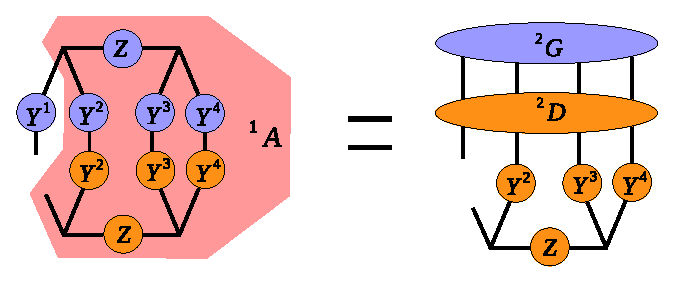
\includegraphics[width=0.6\textwidth]{figures/tcc_theory/cc_thc}}
} .
\label{fig:cc_thc}
\end{equation}
%
Note that the energy denominator ${}^2D$ is represented 
here as an order-8 diagonal tensor ${}^2D^{aba^{\prime} b^{\prime}}_{ij 
i^{\prime} j^{\prime}}$, instead of an order-4 dense tensor ${}^2D^{ab}_{ij}$ 
as in Eqn.~\ref{eq:cc_denom_definition}. The final form of our ALS-type 
coupled cluster doubles equations is provided below (an example for the factor 
$Y^{1}$ is shown; expressions for other factors are analogous):
%
\begin{equation}
\vcenter{\hbox{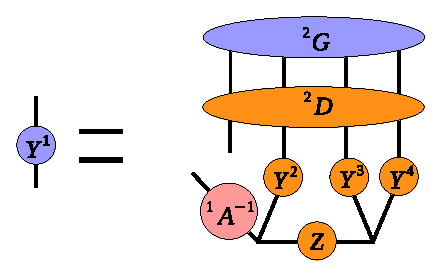
\includegraphics[width=0.4\textwidth]
{figures/tcc_theory/cc_thc_sol}}}.
\label{fig:cc_thc_als}
\end{equation}
%

Here ${}^2G$ on the right hand side is a collection of tensor contractions 
involving the Hamiltonian and THC approximated ${}^2T$ amplitudes 
(see Eqn.~\ref{eq:ccd_amplitude_equation} for the full list of these terms).
We substitute the electron interaction term with its THC decomposition 
calculated beforehand, for example, with ALS. The size of the auxiliary 
dimension in this decomposition is $r_{V}$, and needs to be only of order $O(N)$ 
for a good approximation, as was discussed previously in the section 
\ref{sec:tensor_hypercontraction}. We also substitute the denominator tensor by 
its CP decomposition obtained analytically by means of Laplace transformation. 
The CP rank $r_{D}$ in this decomposition is a small constant $\sim 15$ and 
does not depend on $N$. Finally, we \emph{define} ${}^2T$ amplitudes to have 
THC structure with rank $r_{T}$. The resulting expressions, where all order-4 
tensors are substituted by their decompositions, factorize. After defining 
proper intermediates, the cost of these equations has quartic scaling in 
$r_{V}$, $r_{T}$ and $N$ per iteration. An example of such factorization 
for the contraction we considered before 
in Eqn.~\ref{eq:ccd_intermediate_example2} is 
shown below diagrammatically (we used a dashed line to show an auxiliary 
index in the CP decomposition of ${}^2 D$):
\begin{equation}
\begin{split}
\tau^{ab}_{ij} & = {}^2 T^{cd}_{ij} V^{ab}_{cd} \\
Y^{1 \ast} &\longleftarrow {}^1A^{-1} \cdot \tau \cdot {}^{2}D 
\cdot \frac{\partial ({}^2\tilde{T})}{\partial Y^{1}}
\end{split}
\end{equation}
%
\begin{equation}
\vcenter{\hbox{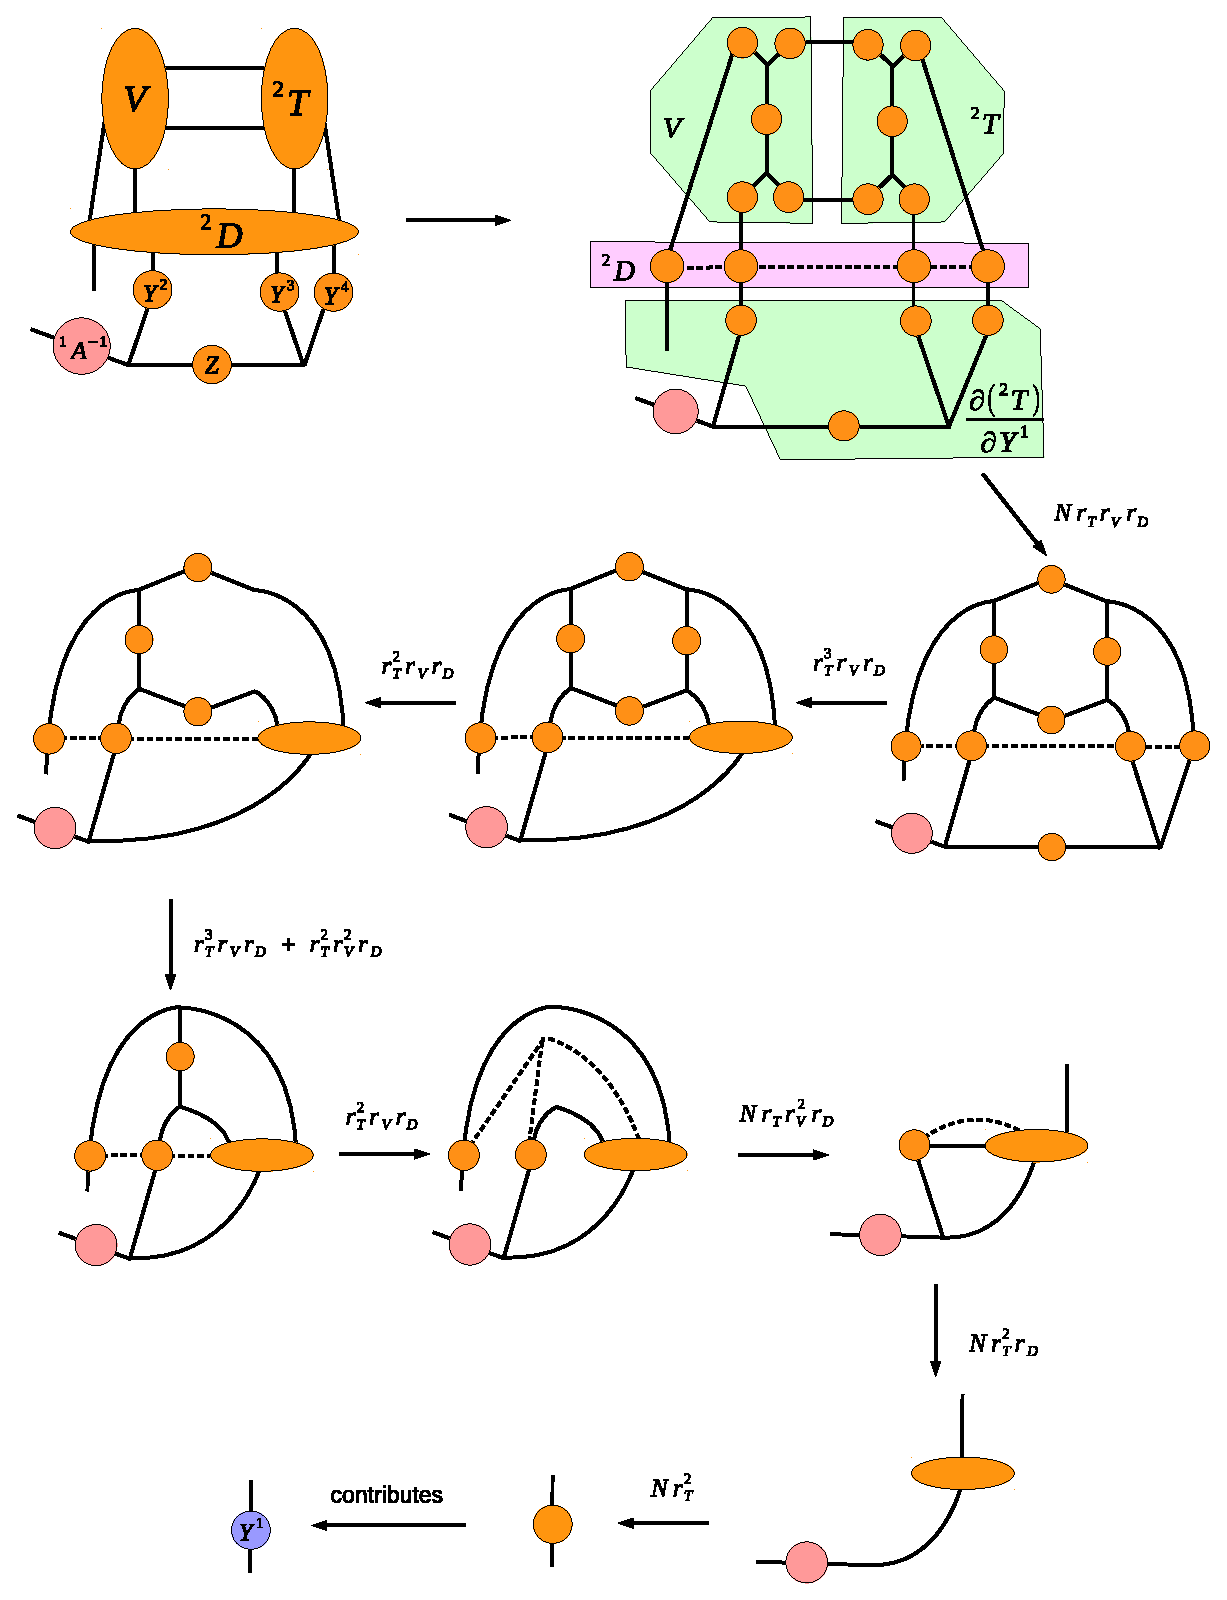
\includegraphics[width=0.95\textwidth]
{figures/tcc_theory/cc_thc_example}}}.
\label{fig:cc_thc_example}
\end{equation}
%
Although diagrams are convenient for explaining tensor factorizations, it 
is still quite challenging to define good intermediates even for the 
simplest decomposed RCCD method. We derived factorized equations using an 
automated algebraic system developed in our group.\cite{drudge1, drudge2} We 
refer the reader to the supplementary material from 
Ref.~\cite{schutski2017tensor} for the complete listing of these expressions for 
the THC decomposed RCCSD method (denoted as THC-RCCSD), as well as their 
implementation in Python.\cite{van2007python}

The algorithm of tensor structured coupled cluster is listed below. 
%
\begin{algorithm}[H]
  \caption{Tensor Structured Coupled Cluster}\label{code:tcc_algorithm}
  \begin{algorithmic}[1] 
  \Function{thc}{$H, r_\mathrm{V}, r_\mathrm{T}, \epsilon_{T}, \epsilon_{E}$}
  \State $F, W^{1},W^{2},\ldots \gets$ approximate\_hamiltonian($H, r_{V}$)
  \State ${}^2D^1,{}^2D^{2},\ldots \gets$ 
Laplace\_transform\_denominator($F$)  
  \State $\tilde{Y}^1, \tilde{Y}^2, \tilde{Y}^3 \ldots \gets$ 
init\_random\_amplitude\_decomposition($r_{T}$) 
  \Repeat 
  \State $Y^1, Y^2, Y^3, \ldots \gets 
$ symmetrize\_amplitudes($\tilde{Y}^{1}, \tilde{Y}^{2}, \tilde{Y}^{3} \ldots$)
   \State $E \gets $ calculate\_cc\_energy($F, W^1, W^2, \ldots, 
\tilde{Y}^{1}, \tilde{Y}^{2}, \ldots$)
  \ForAll {$Y \in \{\tilde{Y}^{1}, \tilde{Y}^{2}, \tilde{Y}^{3}, 
\ldots \}$}
  \State $A_{Y} \gets $ get\_environment($Y^1, Y^2, Y^3, \ldots \tilde{Y}^1, 
\tilde{Y}^2, \tilde{Y}^3, \ldots$)
  \State $B_{Y} \gets $ get\_cc\_rhs($F, W^1, W^2, \ldots, {}^2D^{1}, 
{}^2D^{2}, \ldots Y^{1}, Y^{2}, Y^{3}, \ldots \tilde{Y}^{1}, \tilde{Y}^{2}, 
\ldots$) 
   \State $\tilde{Y}_{new} \gets A^{-1} B$
   \EndFor
   \State $\Delta \gets \max_{Y} \frac{\| \tilde{Y}_{new} - \tilde{Y} \|}{\|
\tilde{Y} \|}$
   \State $\tilde{Y} \gets \tilde{Y}_{new}$ 
   \State $E_{new} \gets $ calculate\_cc\_energy($F, W^1, W^2, \ldots, 
\tilde{Y}^{1}, \tilde{Y}^{2}, \ldots$)
   \State $dE \gets E - E_{new}$
   \Until $\Delta > \epsilon_{T}$ or $dE > \epsilon_{E}$ 
   
   \Return $E, \tilde{Y}^1, \tilde{Y}^2, \tilde{Y}^3, \ldots$
    \EndFunction
  \end{algorithmic}
\end{algorithm}
%
Let us walk though the algorithm. First, a 
decomposition of the two body interaction and the Laplace transformation of 
energy denominators are calculated. Next, the factors in the decomposition of 
amplitudes are initialized with random numbers. For each factor in the 
decomposition of amplitudes its environment and the right hand side in the 
ALS-like equation are calculated (see Eqn.~\ref{fig:cc_thc}). The factors  are 
updated according to Eqn.~\ref{fig:cc_thc_als} until convergence in either the 
coupled cluster energy or the elements of factors is reached.

An important detail of the algorithm is that proper symmetries have to be 
enforced by the decomposition of amplitudes in order for 
the method to converge (See Appendix~\ref{sec:symmetrization} for more 
details). Symmetrization of the decomposition of amplitudes, however, causes 
the growth of decomposition rank $r_{T}$, the situation we would like 
to avoid. This can be done by keeping two sets of amplitudes at each 
iteration. Here we denoted symmetrized factors by $Y$, and their 
unsymmetrized counterparts as $\tilde{Y}$. We used symmetrized factors to 
evaluate ${}^2G({}^2 \tilde{T})$ (see Eqn.~\ref{fig:cc_thc}, dark colored 
shapes), while unsymmetrized factors were used to project ${}^2G({}^2 
\tilde{T}) \cdot {}^2D$ in the ALS-like manner (Eqn~\ref{fig:cc_thc}, light 
colored shapes). This scheme allowed us to keep the rank 
$r_{T}$ fixed from iteration to iteration, while preserving proper symmetries of 
the amplitude tensors, which is required in coupled cluster theory. 

To summarize, equation~\ref{fig:cc_thc_als}, which represents a combination 
of CC and ALS update, is a cornerstone of the tensor structured coupled cluster 
method and the main achievement of this work. Our scheme is quite generic  
and can be applied to any combination of the factorizations of amplitudes and 
the Hamiltonian. In the following sections we will discuss numerical experiments 
with some of those novel methods.


\section{Appendix
\label{sec:Appendix}}
\subsection{Graphical notation
\label{sec:graphical_notation}}
We have extensively used wiring diagrams to represent complicated contractions 
of tensor expressions though the text. This notation is similar to the standard 
diagrams in many-body physics,\cite{mattuck2012guide} but is simpler. We use 
this notation mainly to evaluate the complexity of operations, and also to 
simplify the search for intermediates in complicated expressions.  

In our notations, tensors are represented by shapes.  Typically a
$d$-order tensor is depicted by a polygon with $d$ corners (and a
second-order tensor by a circle), though we have not followed this
convention universally. Indices are denoted by lines; a line
connecting multiple tensors is to be summed over, and open lines
correspond to free indices. If a particular element of a tensor
expression is required, we label the open lines.

As an example, a matrix product would be represented by
%
\begin{equation}
\vcenter{\hbox{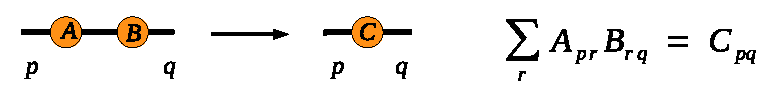
\includegraphics[width=0.7\textwidth]
{figures/tcc_theory/simple_diagrams11}}
}
\end{equation}
%
and a more general contraction of a fourth-order tensor
with a third-order tensor can be shown as
%
\begin{equation}
\vcenter{\hbox{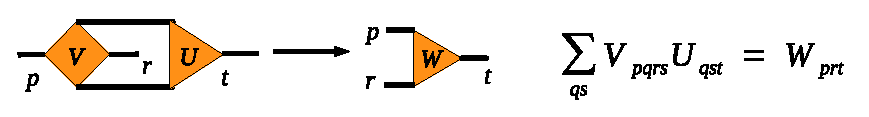
\includegraphics[width=0.7\textwidth]
{figures/tcc_theory/simple_diagrams12}}} .
\end{equation}
%
Diagrams can be used to readily estimate the cost of contractions and
other operations.  The cost $\Omega$ of contracting two tensors over
$L$ indices of size $\{ \lambda \}_1^{L}$ to a tensor with $M$ indices
of size $\{ \mu \}_1^M$ scales with respect to $N$ as
%
\begin{equation} 
\Omega = \mathcal{O}(N^{\sum_{l = 1}^{L} log_{N}
\dim(\{\lambda\}_l) \cdot \sum_{m = 1}^M log_{N} \dim(\{\mu\}_m)}).
\label{eq:contract_scaling_estimate}
\end{equation} 
%
Put simply, the cost of a contraction will scale as $N$ taken to the power of 
the sum of the number of contracted lines and the number of open lines.  
For example, a contraction of two third-order tensors of size $N \times N 
\times N$ over two indices of size $N$ scales as $O(N^4)$:
%
\begin{equation}
\vcenter{\hbox{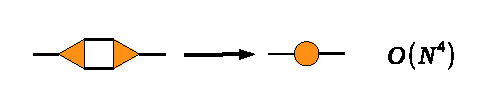
\includegraphics[width=0.6\textwidth]
{figures/tcc_theory/simple_diagrams2}}}
\label{fig:contraction_scaling}
\end{equation}
%
Other operations one may wish to perform on tensors are of outer product type. 
An outer product can be viewed as a contraction over an additional index of 
size one. Diagrammatically, outer products correspond to 
merging the nodes together and leaving all lines in the final structure:
%
\begin{equation}
\vcenter{\hbox{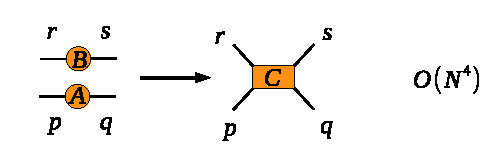
\includegraphics[width=0.5\textwidth]
{figures/tcc_theory/simple_diagrams3}}}
\label{fig:outer_product}
\end{equation} 
%
Note that if one reshapes the fourth-order tensor above
into a matrix with combined indices $rp$ and $sq$, then the result
will coincide with the usual Kronecker product of matrices, where we
recall that the Kronecker product is
%
\begin{equation}
C = A \otimes B \Leftrightarrow C_{rp, sq} = A_{p,q}
\cdot B_{r,s}.
\end{equation}
%
The cost of outer product-type operations is
%
\begin{equation}
\Omega = \mathcal{O}(N^{\sum_{m = 1}^{M} log_{N}
dim(\{\mu\}_m)})
\label{eq:outer_scaling_estimate}
\end{equation}
%
where $\{ \mu \}_1^{M}$ are $M$ free indices in the
resulting tensor.

For our purposes we slightly extended the diagrammatic notation by
introducing summations over an index shared by more than two terms. We
denote such indices by branching lines with a dot at the branching
point. This dot can be interpreted either as an index of the summation
itself, or as a fully diagonal tensor whose elements are contractions
of Kronecker deltas, e.g.
%
\begin{equation} K_{p,q,r,\ldots} = \sum_\alpha \delta_p^\alpha
\delta_q^\alpha \delta_r^\alpha \ldots.
\end{equation}
%
The latter interpretation means that all contractions
in the diagrams can be thought pairwise as in the normal case.
A similar extension has been proposed before in the tensor network 
literature.\cite{ying2016tensor} Using our new
notation, contracting a canonical polyadic decomposition of a third
order-tensor back to a full tensor can be represented as
%
\begin{equation}
\vcenter{\hbox{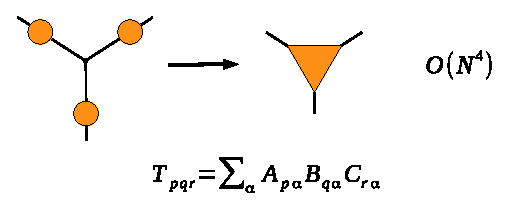
\includegraphics[width=0.5\textwidth]
{figures/tcc_theory/simple_diagrams4}}}
\label{fig:dot_in_diagrams}
\end{equation}
%
If the dimensions of this tensor are $N \times N \times
N$ and the rank of the decomposition (the dimension of the auxiliary
index $\alpha$) is $N$, then the cost of rebuilding the original
tensor from its decomposed form will scale as $O(N^4)$. We note that
Eqn.~\eqref{eq:contract_scaling_estimate} holds in this case just the
same way as with normal pairwise contractions.

Virtually all matrix operations can be seen as either inner or outer 
product, or a combination of them. Let us also provide diagrammatic  
representations of some frequent operations. The Frobenius 
norm of a tensor, which we recall is
%
\begin{equation} \| A \| = \sqrt{\sum_{pqrs \ldots}
A_{pqrs\ldots} \, A^\ast_{pqrs\ldots}},
\end{equation}
%
is given diagrammatically as the square root of a
tensor fully contracted with its own conjugate:
%
\begin{equation}
\vcenter{\hbox{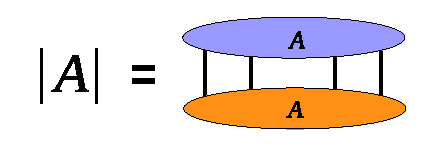
\includegraphics[width=0.3\textwidth]
{figures/tcc_theory/frobenius_norm}}}.
\label{fig:frobenius_norm}
\end{equation}
%
A darker color is used here (as well as in the text) to denote complex
conjugation.

The column-wise Khatri-Rao product is represented by
%
\begin{equation}
D = A \odot B ~~\Leftrightarrow ~~D_{qp,\alpha} =
A_{p,\alpha} \cdot B_{q,\alpha}.
\end{equation}
%
Note that $A$ and $B$ should have the same number of
columns to be compatible. The Khatri-Rao product can be understood as a partial 
outer product over the row indices, while column indices are simply matched. 
The resulting matrix $D$ can be reshaped to a third-order tensor with indices 
$p$, $q$ and $\alpha$. Diagrammatically, the Khatri-Rao product is
%
\begin{equation}
\vcenter{\hbox{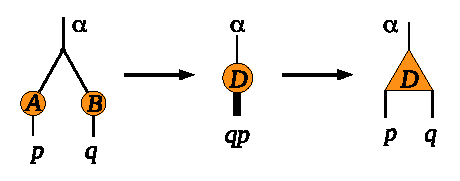
\includegraphics[width=0.5\textwidth]
{figures/tcc_theory/simple_diagrams5}}}.
\label{fig:khatri_rao_product}
\end{equation} 
%
Here we used a thick line to denote a combined index
$qp$. Note also that the canonical polyadic decomposition can be
conveniently expressed through the Khatri-Rao product, which is also
reflected by the diagrams:
%
\begin{equation}
\vcenter{\hbox{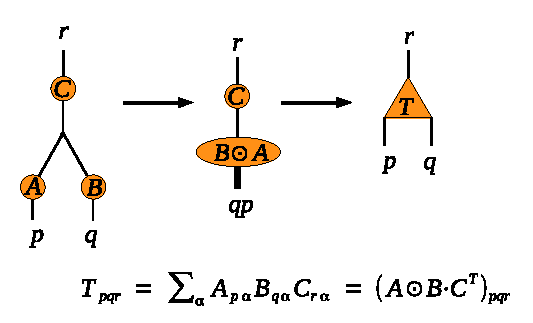
\includegraphics[width=0.6\textwidth]
{figures/tcc_theory/simple_diagrams7}}}
\label{fig:canonical_khatri_rao}
\end{equation}
%
Finally, we point out that wiring diagrams provide an easy way to
calculate derivatives.  A partial derivative of a tensor network with
respect to one of its component tensors is simply the network with
that tensor (but not its lines) removed. On the Figure~\ref{fig:deriv_example}
the derivative of a tensor $T_{ijk} = \sum_{p} A_{ip} B_{jp} C_{kp}$ with 
respect 
to the matrix $A_{mn}$ is shown. We note that one can insert an identity matrix 
$I$ into any edge of a tensor network as this does not alter the result of 
contractions, and also that a disjoint network can be interpreted as a 
Kronecker product of its parts.
%
\begin{equation}
\vcenter{\hbox{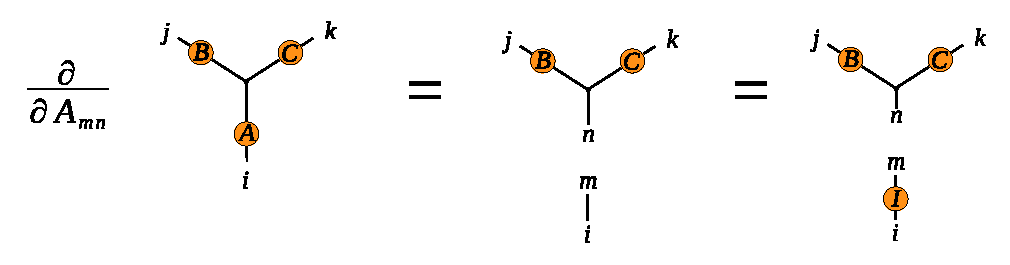
\includegraphics[width=0.9\textwidth]
{figures/tcc_theory/deriv_example}}}
\label{fig:deriv_example}
\end{equation}
%
By making use of the introduced matrix operations one can conclude that 
%
\begin{equation}
 \frac{\partial T}{\partial A} = (B \odot C) \otimes I
\end{equation}
%

\subsection{Symmetrization of tensor decompositions
\label{sec:symmetrization}}
Most of the tensors we used are coefficients of operators, and have to be 
(anti)symmetric with respect to index permutations required by their 
operator algebra. For an arbitrary tensor $\tilde{T}$ its symmetric 
part $T$ can be extracted with the help of the symmetrization operator. 
Lets suppose that $T$ is equivalent under a permutation of indices 
$\{\sigma_{\pi}\}_{\pi=1}^{\Pi}$. The symmetric part of $\tilde{T}$ can then be 
extracted as:
%
\begin{equation}
T_{ijk\ldots} = \frac{1}{\Pi} \sum_{\pi=1}^{\Pi} 
\tilde{T}_{\sigma_{\pi}(i) \sigma_{\pi}(j) \sigma_{\pi}(k) \ldots}
\end{equation}
%
As an example, the double excitation amplitudes in 
RCCD have the following symmetry:
\begin{equation}
 T_{ij}^{ab} = T_{ji}^{ba}
\end{equation}
The double excitation tensor can be symmetrized with the following operation:
%
\begin{equation}
 T_{ij}^{ab} = \frac{1}{2} (\tilde{T}_{ij}^{ab} + \tilde{T}_{ji}^{ba})
 \label{eq:symmetrization}
\end{equation}
%
Preserving proper symmetries of tensors is crucial in many-body methods. 
In the particular case of coupled cluster the violation of the symmetry of 
excitation amplitudes due to numerical noise may quickly lead to divergence of 
the otherwise convergent algorithm (see Figure~\ref{fig:symmetry_convergence}).
%
\begin{figure}[!ht]
\centering
\begin{subfigure}[b]{0.70\textwidth}
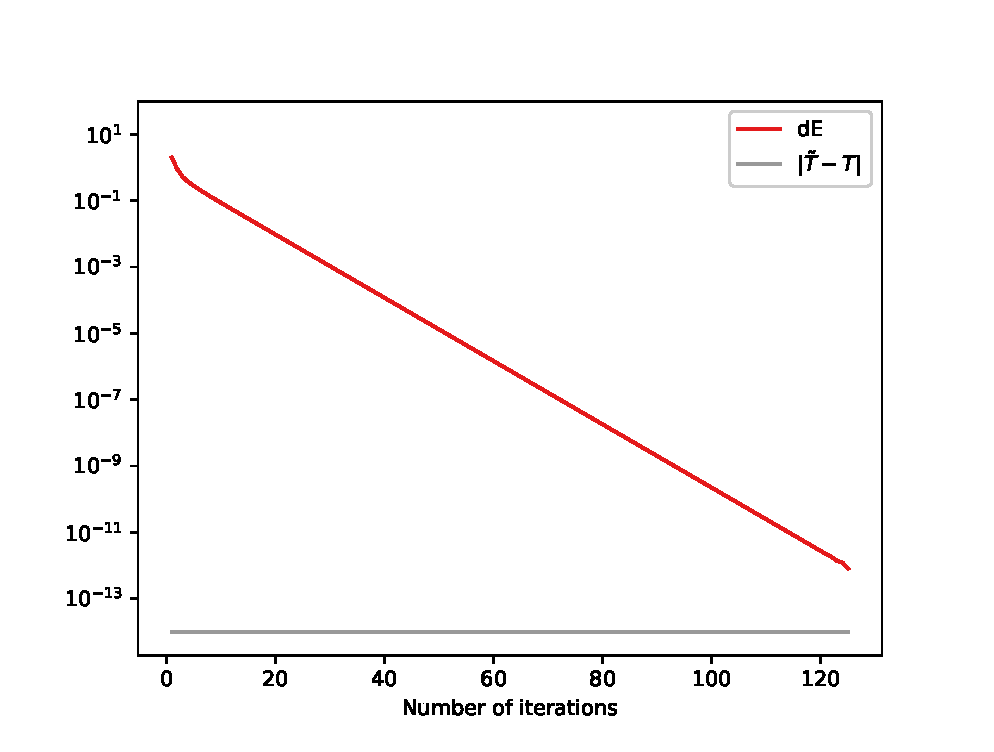
\includegraphics[width=1\linewidth]{figures/tcc_theory/dE_vs_niter_u_3_stable}
   \caption{}
   \label{fig:symmetry_convergence_1} 
\end{subfigure}
\begin{subfigure}[b]{0.70\textwidth}
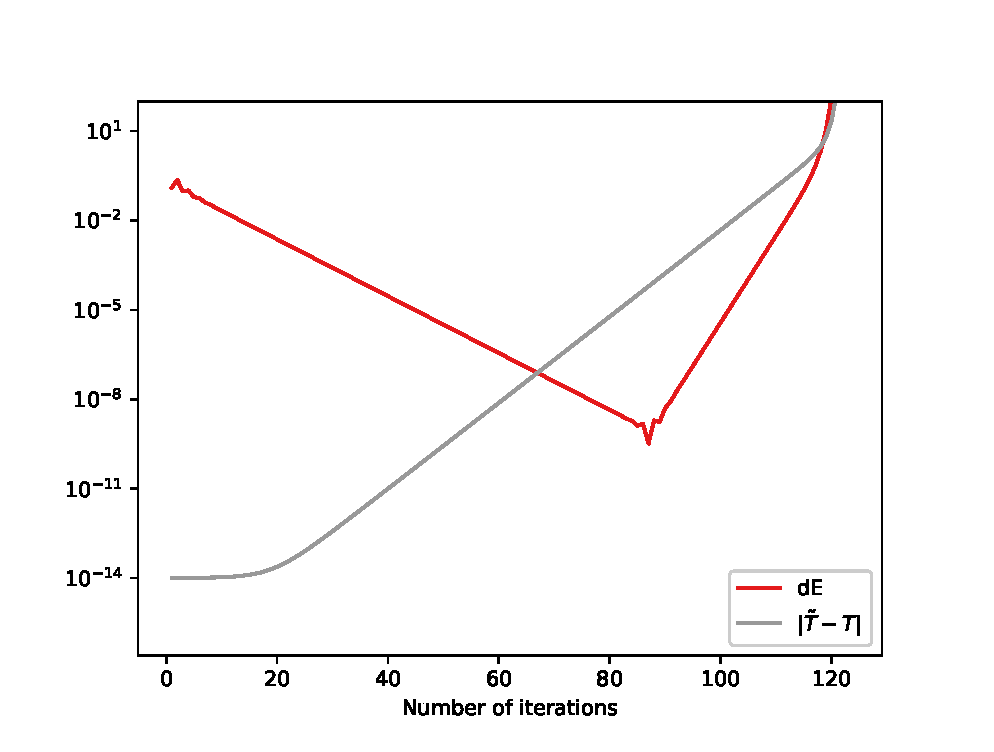
\includegraphics[width=1\linewidth]{figures/tcc_theory/dE_vs_niter_u_3_unst}
   \caption{}
   \label{fig:symmetry_convergence_2}
\end{subfigure}
\caption{Convergence of the RCCD method with (a) and without (b) enforcing the 
symmetry of ${}^2 T$ amplitudes. The lower panel shows the divergence of RCCD 
iterations due to the accumulation of numerical noise, while the same algorithm 
converges to machine precision if the noise is eliminated.}
\label{fig:symmetry_convergence}
\end{figure}
%
Decompositions of higher order tensors, however, are usually not constrained 
to strictly preserve permutation symmetries. It is important though to provide 
a way of symmetrizing tensor decompositions \emph{directly} (e.g. without 
rebuilding high order tensors, as this will eliminate all benefits of the 
decomposition).

\subsubsection{Canonical decomposition}
Canonical decomposition can be symmetrized by using its summation and 
permutation properties.
\begin{itemize}
  \item For a tensor $T$ having a canonical decomposition $T_{ijk} = \sum_{p} 
A_{ip} B_{ip} C_{jp}$ its permutations can be built by simply permuting the 
order of factors in the summation.
  \item If tensors $T$ and $U$ both have canonical decompositions with ranks 
$r_{T}$ and $r_{U}$ respectively, then their sum is a canonical decomposition 
with rank $r = r_{T} + r_{U}$. This means that the factor matrices of $T$ and 
$U$ can be concatenated column-wise:
%
\begin{equation}
\begin{aligned}
 T_{ijk} &= \sum_{p=1}^{r_{T}} A_{ip} B_{jp} C_{kp}, \qquad U_{ijk} = 
\sum_{p=1}^{r_{U}} D_{ip} E_{jp} F_{kp} \\
(T + U)_{ijk} &= \sum_{p=1}^{r_{T} + r_{U}} (A | D)_{ip} (B | E)_{jp} (C | 
F)_{kp}
\end{aligned}
\end{equation}
where we used $(A | D)$ to denote a column-wise concatenation of matrices $A$ 
and $D$
\end{itemize}
 
Using the properties of the CPD it is possible to symmetrize tensors directly 
in their decomposed form. Suppose that an amplitude tensor has a 
canonical decomposition:
%
\begin{equation}
 \tilde{T}_{ij}^{ab} = \sum_{p=1}^{P} W^{1}_{ap} W^{2}_{bp} 
W^{3}_{ip} W^{4}_{jp}
\end{equation}
%
Then the symmetric part of $T$ can be 
represented as:
%
\begin{equation}
\begin{aligned}
 T_{ij}^{ab} &= \frac{1}{2} (\tilde{T}_{ij}^{ab} + \tilde{T}_{ji}^{ba}) \\
 T_{ij}^{ab} &= \frac{1}{2} \sum_{p=1}^{2P} (W^{1} | W^{2})_{ap} (W^{2} | 
W^{1})_{bp} (W^{3} | W^{4})_{ip} (W^{4} | W^{3})_{jp} 
\end{aligned}
\end{equation}
%
the normalization scalar can be absorbed into one of the new factors. We note 
that the symmetrized decomposition may not have an optimal rank (e.g. 
CPD with a lower rank and same accuracy may exist), but this growth of rank did 
not pose a problem in our applications.

\subsubsection{Tensor Hypercontraction}
The symmetrization expressions in case of THC factorization can be build 
using an analogous reasoning. If a tensor $\tilde{T}$ has a 
THC decomposition $\tilde{T}_{ij}^{ab} = \sum_{pq} W^{1}_{ap} W^{2}_{ip} X_{pq} 
W^{3}_{bq} W^{4}_{jq}$, then it can also be regarded having a CP decomposition 
with a "thick" factor $Q_{R}$, as is shown below:
%
\begin{equation}
\vcenter{\hbox{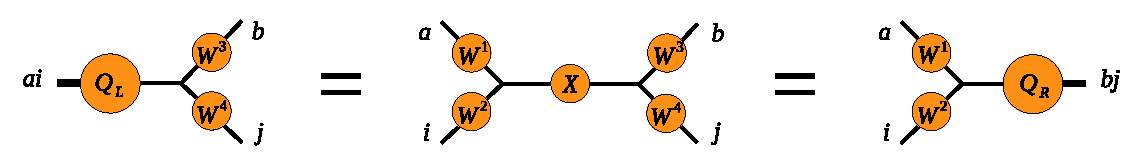
\includegraphics[width=0.9\textwidth]
{figures/tcc_theory/thc_as_cpd_sym}}}.
\label{fig:thc_as_cpd_sym}
\end{equation}
%
The same is true for the left part of the THC tensor network. The final 
result of the symmetrization is:
%
\begin{equation}
\begin{aligned}
 T_{ij}^{ab} &= \frac{1}{2} (\tilde{T}_{ij}^{ab} + \tilde{T}_{ji}^{ba}) \\
 T_{ij}^{ab} &= \frac{1}{2} \sum_{p=1}^{2P}\sum_{q=1}^{2Q} (W^{1}|W^{3})_{ap} 
(W^{2}|W^{4})_{ip} \left(
\begin{array}{c|c}
X & 0 \\
\hline
0 & X^{T}
\end{array}
\right)_{pq} (W^{3}|W^{1})_{bq} (W^{4}|W^{2})_{jq}  
\end{aligned}
\label{eq:thc_symmetrization}
\end{equation}
%
As one may notice from Eqn.~\ref{eq:thc_symmetrization}, the number 
of elements in the factor $X$ grows as a square of the number of symmetry 
operations. This happens because the symmetry $T_{ij}^{ab} = T_{ji}^{ba}$ 
permutes pairs of indices ($ai$ and $jb$) located farther away from each other 
compared to CPD. It follows again that the structure of the decomposition plays 
a crucial role in what tensors the decomposition can effectively approximate.
